\documentclass[a4paper, 14pt]{extarticle}%тип документа

\date{}

\usepackage{graphicx}
\usepackage{cmap}
\usepackage[T2A]{fontenc}
\usepackage[utf8]{inputenc}
\usepackage{indentfirst}


\usepackage[english,russian]{babel}
\usepackage{multirow} % Слияние строк в таблице
\newcommand
{\un}[1]
{\ensuremath{\text{#1}}}

%Русский язык
\usepackage[T2A]{fontenc} %кодировка
\usepackage[utf8]{inputenc} %кодировка исходного кода
\usepackage[english,russian]{babel} %локализация и переносы

%Таблицы
\usepackage[table,xcdraw]{xcolor}
\usepackage{booktabs}

%Математика
\usepackage{amsmath, amsfonts, amssymb, amsthm, mathtools}

%отступы 
\usepackage[left=2cm,right=2cm,top=2cm,bottom=3cm,bindingoffset=0cm]{geometry}

%Графики
\usepackage{pgfplots}
\pgfplotsset{compat=1.9}

%Вставка картинок
\usepackage{graphicx}
\usepackage{wrapfig, caption}
\graphicspath{}
\DeclareGraphicsExtensions{.pdf,.png,.jpg, .jpeg}
\newcommand\ECaption[1]{%
\captionsetup{font=footnotesize}%
\caption{#1}}

\captionsetup{labelformat=empty,labelsep=none}

\usepackage{blindtext}
\usepackage{hyperref}

\begin{document}

% НАЧАЛО ТИТУЛЬНОГО ЛИСТА

\begin{titlepage}
	\begin{center}
		\large 	Московский физико-технический университет \\
		Физтех-школа радиотехники и компьютерных технологий\\
		\vspace{0.2cm}
		
		\vspace{4.5cm}
		Эссе на тему:  \\ \vspace{0.2cm}
		\LARGE \textbf{"Развитие квантовой криптографиии в России"}
	\end{center}
	\vspace{2.3cm} \large
	
	\begin{center}
		Работу выполнил: \\
		Шурыгин Антон \\
		Б01-909

	\end{center}
	
	\begin{center} \vspace{60mm}
		г. Долгопрудный \\
	\end{center}
\end{titlepage}

% КОНЕЦ ТИТУЛЬНОГО ЛИСТА

\newpage
\thispagestyle{plain}
\tableofcontents
\thispagestyle{plain}
\newpage

\section{Вступление}

Рассказывая о последних достижениях квантовой крипторафии в России, невозможно обойти стороной понятие "квантовая криптография" в целом как явление.
Почему квантовая? И причем тут вообще криптография? На эти и другие вопросы постараюсь ответить во кратком введении обо всём и ни о чем.

\section{Историческая справка}

Первая идея предложить защищать информацию, используя квантовые понятия и объекты, принадлежит Стивену Визнеру. 
А именно в 1970 году аспирант Колумбийского института выдвинул идею квантового сопряженного кодирования (что также называют квантовым кодированием или квантовым мультплексированием), 
предположив, что отдельные полязированные фотоны можно удачно использовать для кодирования информации. Впоследствии идея \textbf{"сопряженного кодирования"} получила свое продолжения для моделирования квантовых денег в лабораторных условиях, а в мире зародилось новое понятие, которое мы сейчас называем \textbf{"квантовая криптография"}. 

Почти десять лет спустя Чальз Беннет и Жиль Бассар, зная о работе Визнера, предложили передавать секретный ключ с использованием кватонвых объектов. И чуть позже, в 1984, ими была изобретена схема \textbf{BB84} - первый протокол квантовой криптографии, в котором известные порядочные персонажи, Алиса и Боб, обмениваются сообщениями в виде поляризованных фотонов по квантовому каналу. 

Сейчас у вас закономерно могут возникать вопросы. Что за "поляризация"? Какой еще "квантовый канал"?
Постараюсь ответить на эти и другие вопросы, вкратце рассказав о протоколе \textbf{BB84}. 


\begin{figure}[h!]
    \begin{center}
    \begin{minipage}[h]{0.4\linewidth}
        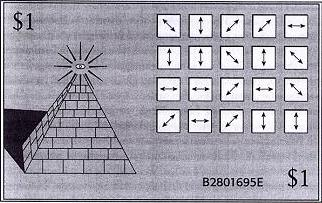
\includegraphics[width=1\linewidth]{pics/quantum_money.jpg}
        \caption{Эскиз квантовой банкноты Стивена Визнера} 
    \label{} 
    \end{minipage}
\hfill
    \begin{minipage}[h]{0.5\linewidth}
        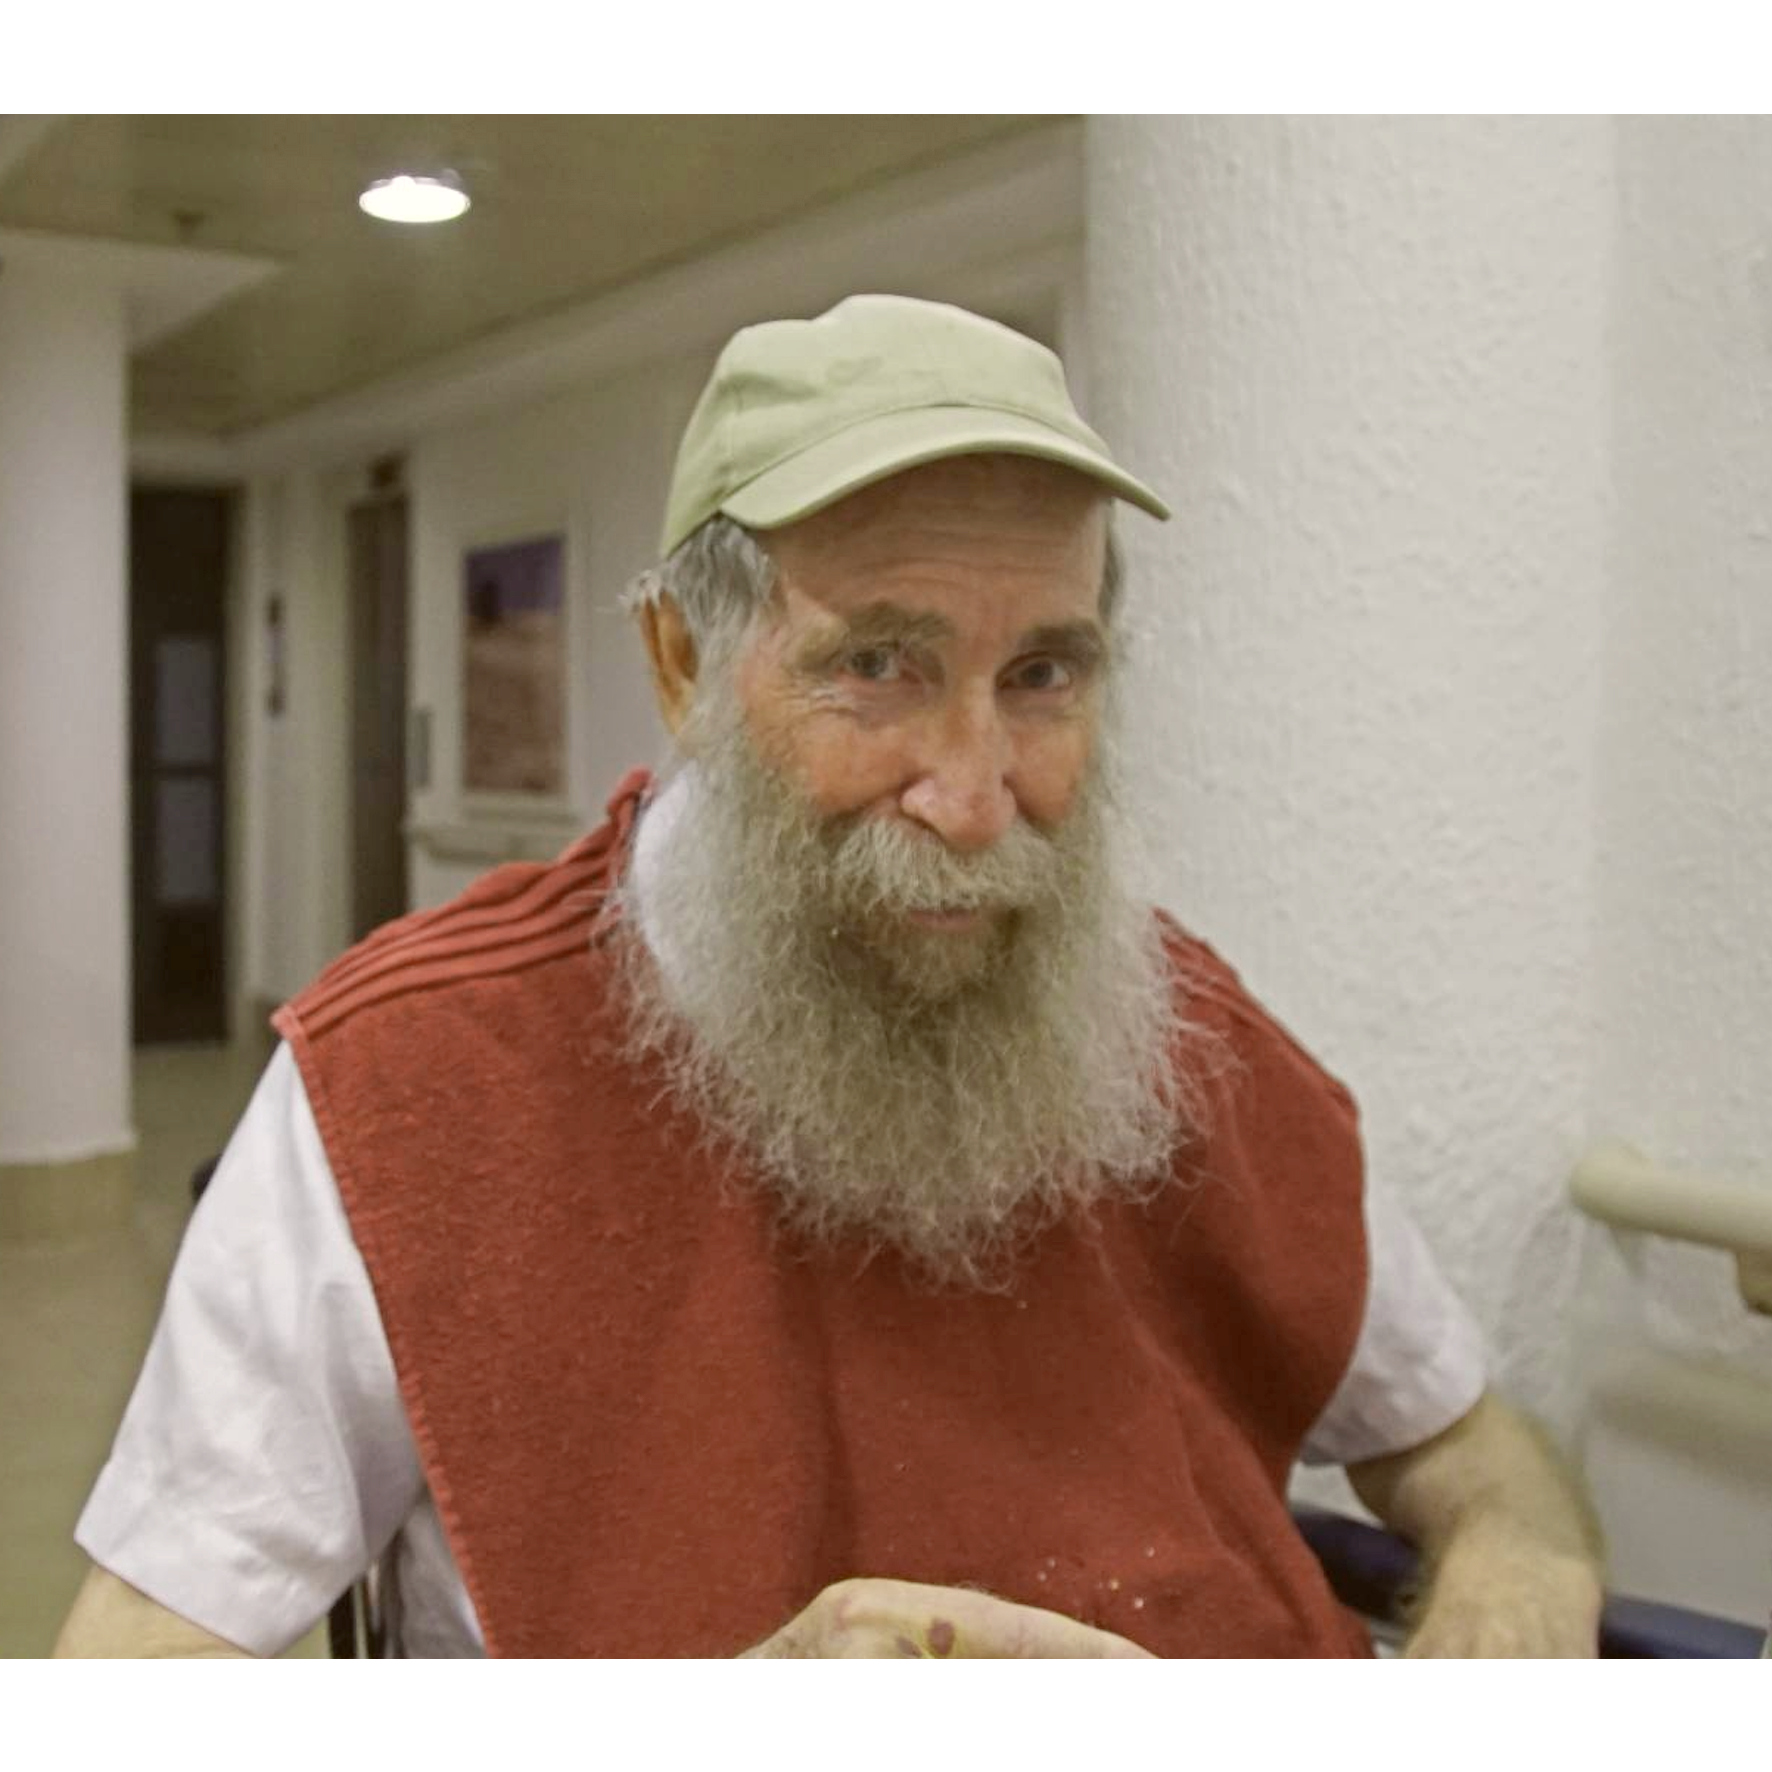
\includegraphics[width=1\linewidth]{pics/Stephen_Wiesner.jpg}
        \caption{Стивен Визнер}
        \label{}
    \end{minipage}
    \end{center}
\end{figure}

% \newpage

\section{Введение в квантовую криптографию}

История криптографии основана на постоянном противостоянии криптографов и крипитоаналитиков. Одни придумывают методы шифрования и защиты информации, а другие - взламывают. 
Стоит отдать должное, что в теории победа именно за криптографами, так как существуем соврешенно невзламываемая штука - одноразовый блокнот (например, шифр Вернама). 
Однако как и у одноразовых блокнотов, так и просто у очень сложных алгоритмов шифрования есть одна общая проблема - распределение ключей.
Однако криптографы не стояли на месте и в 1976 году появился \textbf{протокол Диффи - Хеллмана} -  протокол обмена ключами, позволявший получить общий секретный ключ, используя открытый канал связи. 
Протокол был основан на гипотезе того, что обратная задача дискретного логарифмирования - большая проблема. Потому надеждность алгоритма высокая лишь до тех пор, пока хакеры не научатся быстро и эффективно находить дискретный логарифм.

И может это все пошатнуться именно в момент, когда реализуют достаточно мощный квантовый компьютер. А все потому что в 1994 году \textbf{Питер Шор} разработал квантовый алгоримт факторизации (или же разложение числа на простые множители). Алгоритм позволяет разложить число $M$ за время $O(log^{3} (M))$, используя $O(log(M))$ логических кубитов. А в догонку к этой задаче разработанный алгоритм и проблему поиска обратного логарифма может решить. 
Таким образом, американский ученый заставил \textbf{потенциально} уничтожил и асимметричную криптографию RSA и симметричную - Диффи - Хеллмана. 

\begin{figure}[h!]
    \begin{center}
    \begin{minipage}[h]{0.3\linewidth}
        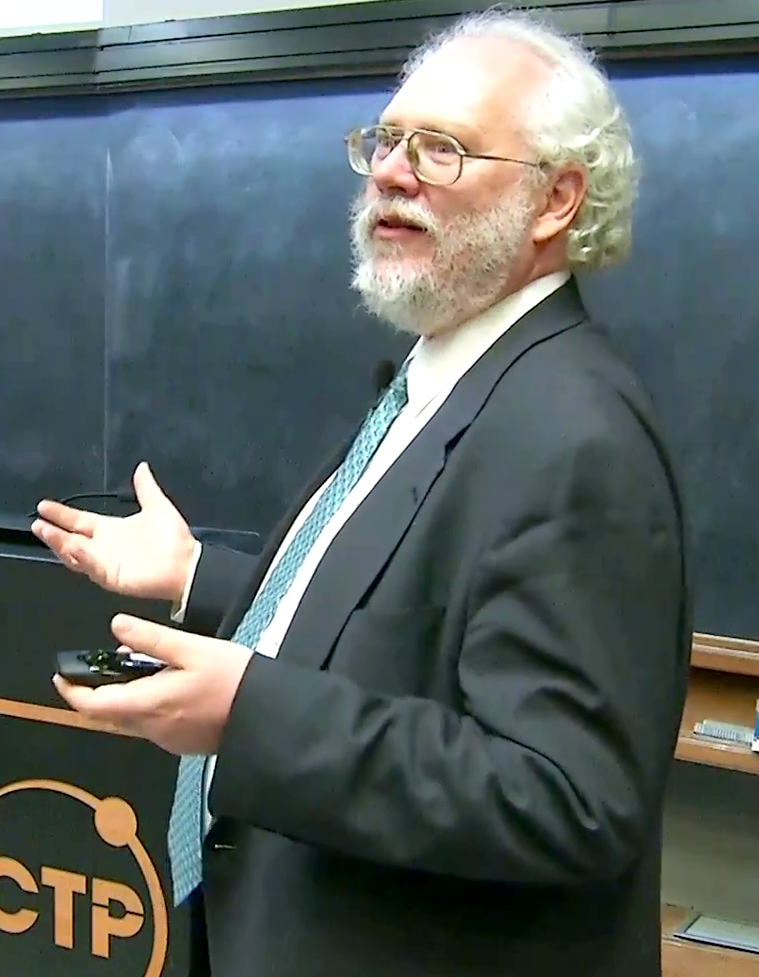
\includegraphics[width=1\linewidth]{pics/Peter_Shor.png}
        \caption{Питер Шор на конференции} 
    \label{} 
    \end{minipage}
\hfill
    \begin{minipage}[h]{0.6\linewidth}
        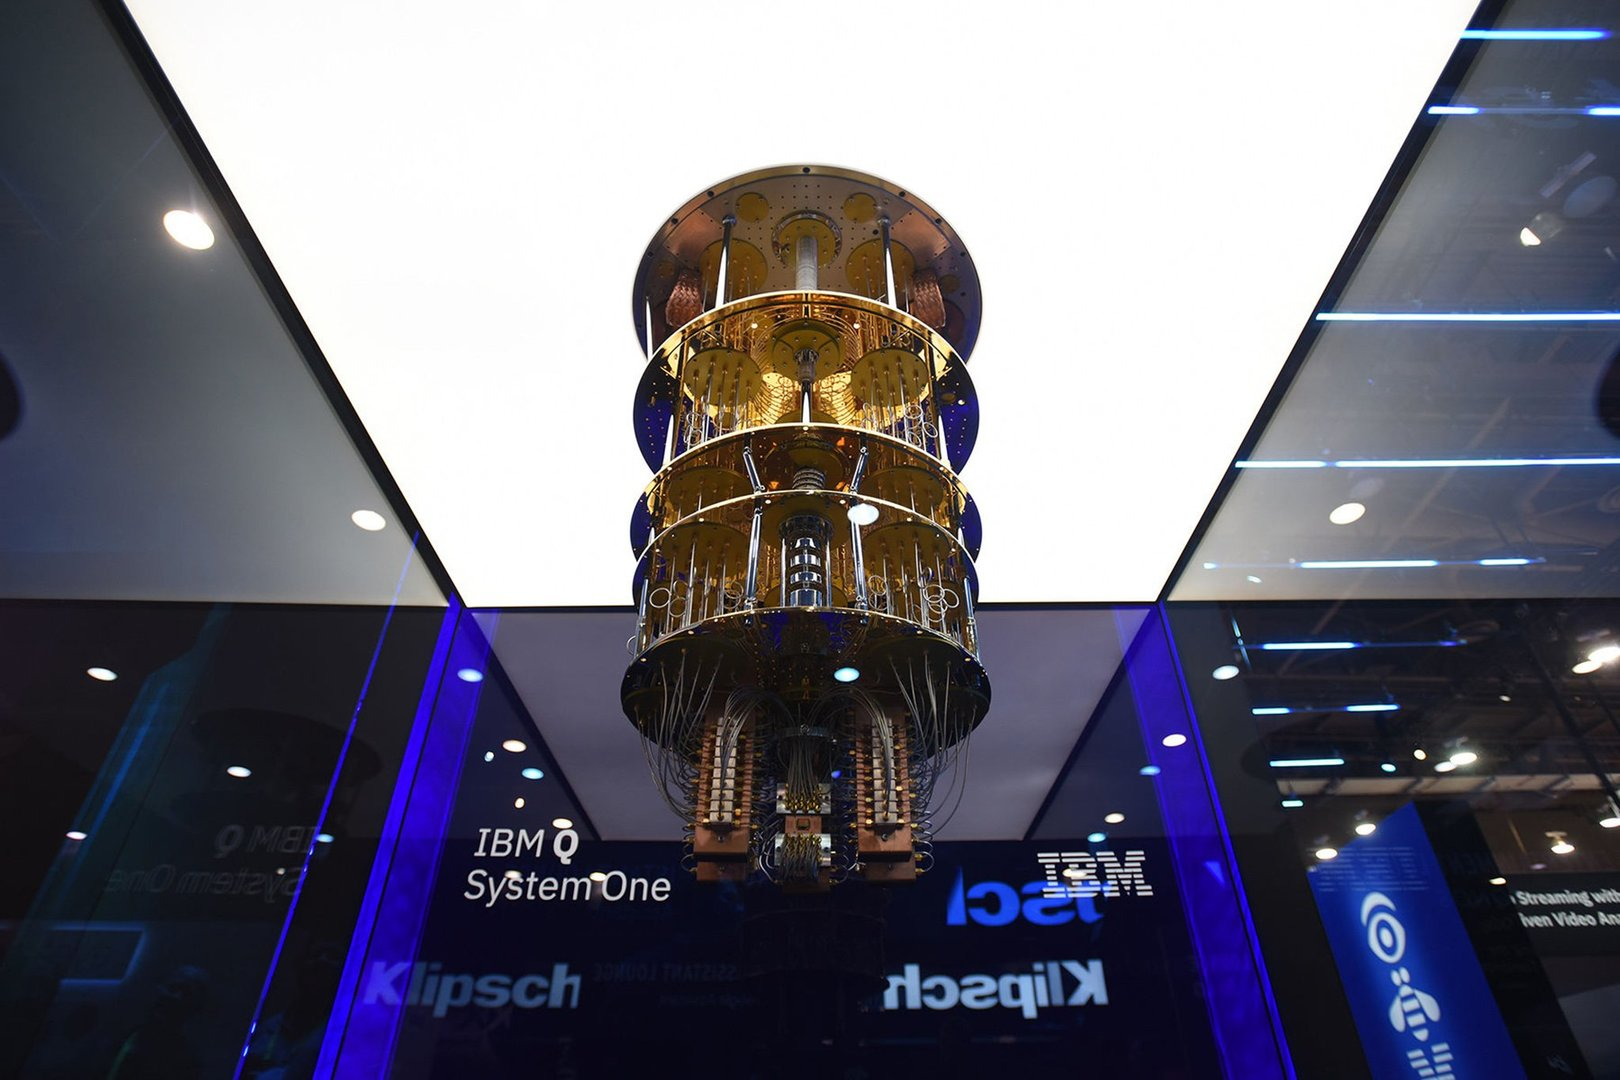
\includegraphics[width=1\linewidth]{pics/IBM_quantum_computer.jpg}
        \caption{Первый коммерческий квантовый комьютер от IBM, 20-кубитная система Q System One, CES 2019}
        \label{}
    \end{minipage}
    \end{center}
\end{figure}

Отнюдь ученые снова не сидели сложа руки, и именнно квантовая критпография позволила придумать новый способ распределения ключей, в котором нет тех проблем, которые, например, присуще схеме Диффи - Хеллмана (например, уязвимость перед простой атакой Man In The Middle).
Речь идет именно про \textbf{BB84}. Безусловно, есть более сложные, более современные алгоритмы такие, как B92, SARG04, Lo05 и так далее. Но для базового понимания того, что вообще происходит, проще всего рассмотреть именно BB84.

\section{Вкратце о BB84}

Алиса может последовательно посылать Бобу фотоны, каждый имеет одно из четырех возможных квантовых состояний (поляризаций):  $\uparrow$, $\rightarrow$, $\nearrow$, $\nwarrow$. 
Эти 4 состояния образуют 2 ортогональных базиса. Состояния внутри одного базиса ортогональны, состояния из разных базисов - попарно неортогональны. 
Боб проводит измерения устройствами с двумя возможными конфигурациями: $\oplus$ , $\otimes$. В какой именно поляризации послать очередной фотон выбирается на основании случайного выбора. В идеальной ситуации это должен быть истинно случайный процесс.

\begin{table}[h!]
    \centering
    \begin{tabular}{| c | c | c |}
    \hline
    $ Обозначение $ & Поляризация фотонов        & Бит \\
    \hline
    $\uparrow$      & Горизонтальная             & $1$  \\
    \hline  
    $\rightarrow$   & Вертикальная               & $0$  \\
    \hline  
    $\nearrow$      & Под углом $\frac{\pi}{4}$    & $0$  \\
    \hline  
    $\nwarrow$      & Под углом $\frac{3\pi}{4}$   & $1$   \\
    \hline  

    \end{tabular}
    \caption{Условные обозначения}
\label{tb1}
\end{table}

Отсюда получаются очевидные соотношения для вероятостей измерения:
\begin{multline}
    \\
    P(\uparrow | \oplus) = 1,\:\: P(\rightarrow | \oplus) = 1                           \\
    P(\uparrow | \otimes) = \frac{1}{2}, \:\: P(\rightarrow | \otimes) = \frac{1}{2}    \\
    P(\nearrow | \otimes) = 1,\:\: P(\nwarrow | \otimes) = 1                           \\
    P(\nearrow | \oplus) = \frac{1}{2}, \:\: P(\nwarrow | \oplus) = \frac{1}{2}    \\
\end{multline}

% $\uparrow$, $\rightarrow$, $\nearrow$, $\nwarrow$
% $\oplus$ , $\otimes$

\subsection{BB84 без злоумышленника}

\begin{enumerate}
    \item Алиса случайно выбирает один из базисов. Затем внутри базиса случайно выбирает одной из состояний, соответствующее либо 0, либо 1. Посылает фотоны. 
    \item Для каждого фотона Боб случайно и незавимисо от Алисы выбирает один из приборов и измеряет поляризацию пришедшего фотона. 
    \item Боб связывается с Алисой по открытому каналу и сообщает ей, какие приборы он использовал для измерения последовательности фотонов.
    \item В ответ Алиса сообщает, в каких случаях был выбран правильных прибор и соответственно базис. 
    \item Вычеркивается неверно измеренные фотоны. Оставшаяся часть, последовательность нулей и единиц - есть секретный ключ. 
\end{enumerate}

\subsection{Пример 1}

\begin{table}[h!]
    \centering
    \begin{tabular}{| c | c | c | c | c | c | c | c | c |}
    \hline
    от Алисы       & $\nearrow$ & $\nearrow$ & $\rightarrow$ & $\uparrow$ & $\uparrow$ & $\rightarrow$ & $\nwarrow$ & $\nwarrow$ \\
    \hline
    Приборы Боба   & $\oplus$ & $\otimes$ & $\oplus$ & $\oplus$ & $\otimes$ & $\otimes$ & $\otimes$ & $\oplus$ \\
    \hline
    Результат Боба & $\rightarrow$ & $\nearrow$ & $\rightarrow$ & $\uparrow$ & $\nearrow$ & $\nearrow$ & $\nwarrow$ & $\uparrow$ \\
    \hline
    Биты           &  & 0 & 0 & 1 &  &  & 1 &  \\
    \hline
\end{tabular}

% $\uparrow$, $\rightarrow$, $\nearrow$, $\nwarrow$. 
% $\oplus$ , $\otimes$
    \caption{Пересылка без Евы}
    \label{tb2}
\end{table}

Итоговая последовательность: \textbf{0011} - есть секретный ключ.

\subsection{BB84 с злоумышленником}

Так же вкратце рассмотрим ситуацию, при которой между Алисой и Бобом есть злоумышленник - Ева. 

\begin{enumerate}
    \item Ева пытается перехватить биты через квантовый канал, как и Боб, случайно выбирая поляризацию. В отличие от Боба она не сможет после передачи синхронизироваться с Алисой и уточнить, правильный ли базис она выбрала для каждого фотона. 
    \item В случае неправильно угаданных поляризаций, Ева будет ``портить`` волновые функции передаваемых фотонов (принцип неопределенности Гейзенберга). В итоге пересылаемая Бобу последовательность с \textbf{очень большой вероятностью} будет уже совсем не той, которую он должен был получить изначально. 
    \item Далее все так же. Боб связывается с Алисой, сверяют использованные приборы. Боб вычеркивает биты, однако в итоге у него получится другая последовательность бит, нежели у Алисы. 
\end{enumerate}

\subsection{Пример 2}

\begin{table}[h!]
    \centering
    \begin{tabular}{| c | c | c | c | c | c | c | c | c |}
    \hline
    от Алисы       & $\nearrow$ & $\nearrow$ & $\rightarrow$ & $\uparrow$ & $\uparrow$ & $\rightarrow$ & $\nwarrow$ & $\nwarrow$ \\
    \hline
    Приборы Евы    & $\oplus$ & $\oplus$ & $\otimes$ & $\otimes$ & $\otimes$ & $\otimes$ & $\otimes$ & $\oplus$ \\
    \hline
    от Евы         & $\uparrow$ & $\rightarrow$ & $\nwarrow$ & $\nwarrow$ & $\nearrow$ & $\nwarrow$ & $\nwarrow$ & $\rightarrow$ \\
    \hline
    Приборы Боба   & $\oplus$ & $\otimes$ & $\oplus$ & $\oplus$ & $\otimes$ & $\otimes$ & $\otimes$ & $\oplus$ \\
    \hline
    Результат Боба & $\uparrow$ & $\nwarrow$ & $\rightarrow$ & $\uparrow$ & $\nearrow$ & $\nwarrow$ & $\nwarrow$ & $\rightarrow$ \\
    \hline
    Биты           &  & 1 & 0 & 1 &  &  & 1 &  \\
    \hline
\end{tabular}

% $\uparrow$, $\rightarrow$, $\nearrow$, $\nwarrow$. 
% $\oplus$ , $\otimes$
    \caption{Пересылка с Евой}
    \label{tb3}
\end{table}

Итоговая последовательность: \textbf{1011} - есть секретный ключ.

Но как Алиса и Боб могут удостовериться, что передача действительно была секретной?

Решение есть. 
\begin{itemize}
    \item Алиса и Боб выбирают в своей последовательности $n$ бит, которые будут сравнивать по \textbf{открытому каналу}.
    \item Если все биты совпали, с вероятносью $P = 1 - 2^{-k}$ канал не прослушивается. Использованные для проверки $n$ бит отбрасываются.
    \item Критической величиной ошибки является 11 \% $\Rightarrow $ значит, Ева пыталась перехватить сообщение. Тогда перепроверяют квантовый канал и начинают заново.  
\end{itemize}

\subsection{Практическая реализация}

Экспериментальная схема представлена на рисунке.

\begin{figure}[h!]
    \centering
    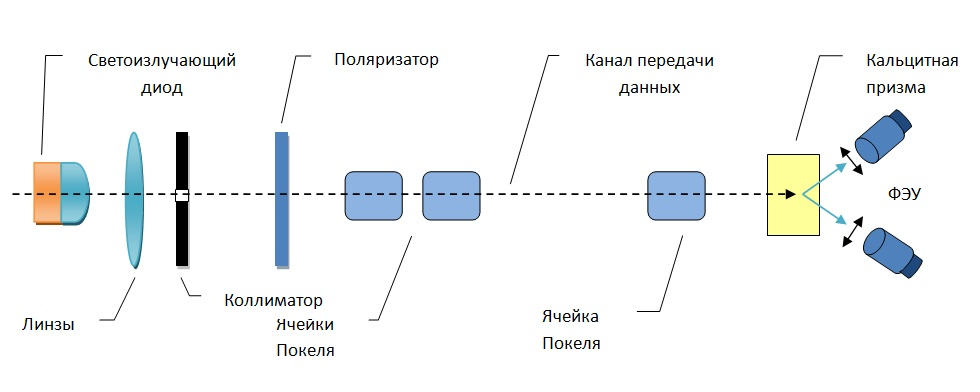
\includegraphics[width=1.0\linewidth]{pics/bb84_realisation.jpg}
    \caption{Практическая реализация протокола BB84}
    \label{scheme}
\end{figure}


\section{Развитие квантовой криптографии в России}

Я постарался вас убедить в том, что квантовая криптография совсем не фантастический раздел современной науки, а вполне реальный метод защиты коммуникации, который наверняка активно будет использоваться в будущем.
Разобрвашись немного в этом вопросе и случайно наткнувшись на пару статей касательно современных достижений в области квантовой криптографии, захотелось узнать, а что же полезного и актуального происходит в российской науке в этой области.

\subsection{МФТИ $\times$ НИТУ МИСиС}

Будучи студентом МФТИ, невозможно начать данный список с какой-либо другой актуальной разработки, пусть она и косвенно относится к квантовой криптографии.  

16 ноября 2022 года команда ученых из МФТИ и НИТУ МИСиС создала четырехкубитных квантовый процессор и продемонстрировала на нем точность двухкубиных операций $CZ$ более 97 \%.

\begin{figure}[h!]
    \centering
    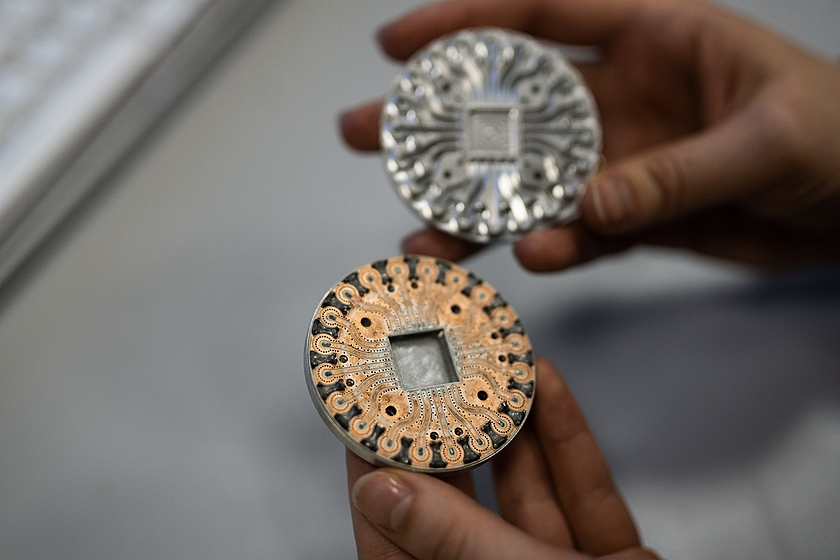
\includegraphics[width=0.8\linewidth]{pics/quantum_processor.jpg}
    \caption{Квантовый процессор, разработанный в МФТИ}
    \label{missis_lab}
\end{figure}

В эксперименте использовалась разработанная и изготовленная сотрудниками Лаборатории искусственных квантовых систем МФТИ сверхпроводниковая интегральная квантовая микросхема, первые готовые образцы которой были изготовлены еще в марте 2021 года. Данное событие, безусловно, является уникальным достижением для российских кватонвых технологий. 
В проведенном эксперименте время отдельной логической операции составляет около 0.025 мкс. Это позволяет реализовать более 3200 операций за время жизни квантового состояния процессора 

\subsection{QApp}

Компания занимается разработкой программных решений на основе постквантовой криптографии. 

\textbf{Постквантовая криптография} - это набор алгоритмов ассиметричной криптографии, взлом которых с помощью квантовых компьюетров не возможен. 

Имеет те же интерфейсы, что и нынешние классические решения ассиметричной криптографии и сопоставимые нефункциональные характеристики работы (скорость, размеры ключей).
Компания активно сотрудничает с российскими производителями микроэлектроники (``Эльбрус'', ``Байкал'') и встраивает свои продукты (библиотеки, пакеты) в их решения. Так, например, была разработана \textbf{PQLR SDK} - интегрированная с OpenSSL криптографическая библиотека, состоящая из самых акутальных квантово-устойчивых алгоритмов, совместима с отечественными процессорами ``Байкал''.

В России, в рамках подгрупп ТК26, сотрудники компании QApp ведут активную деятельность по формированию подходов к стандартизации постквантовой криптографии.

\begin{figure}[h!]
    \centering
    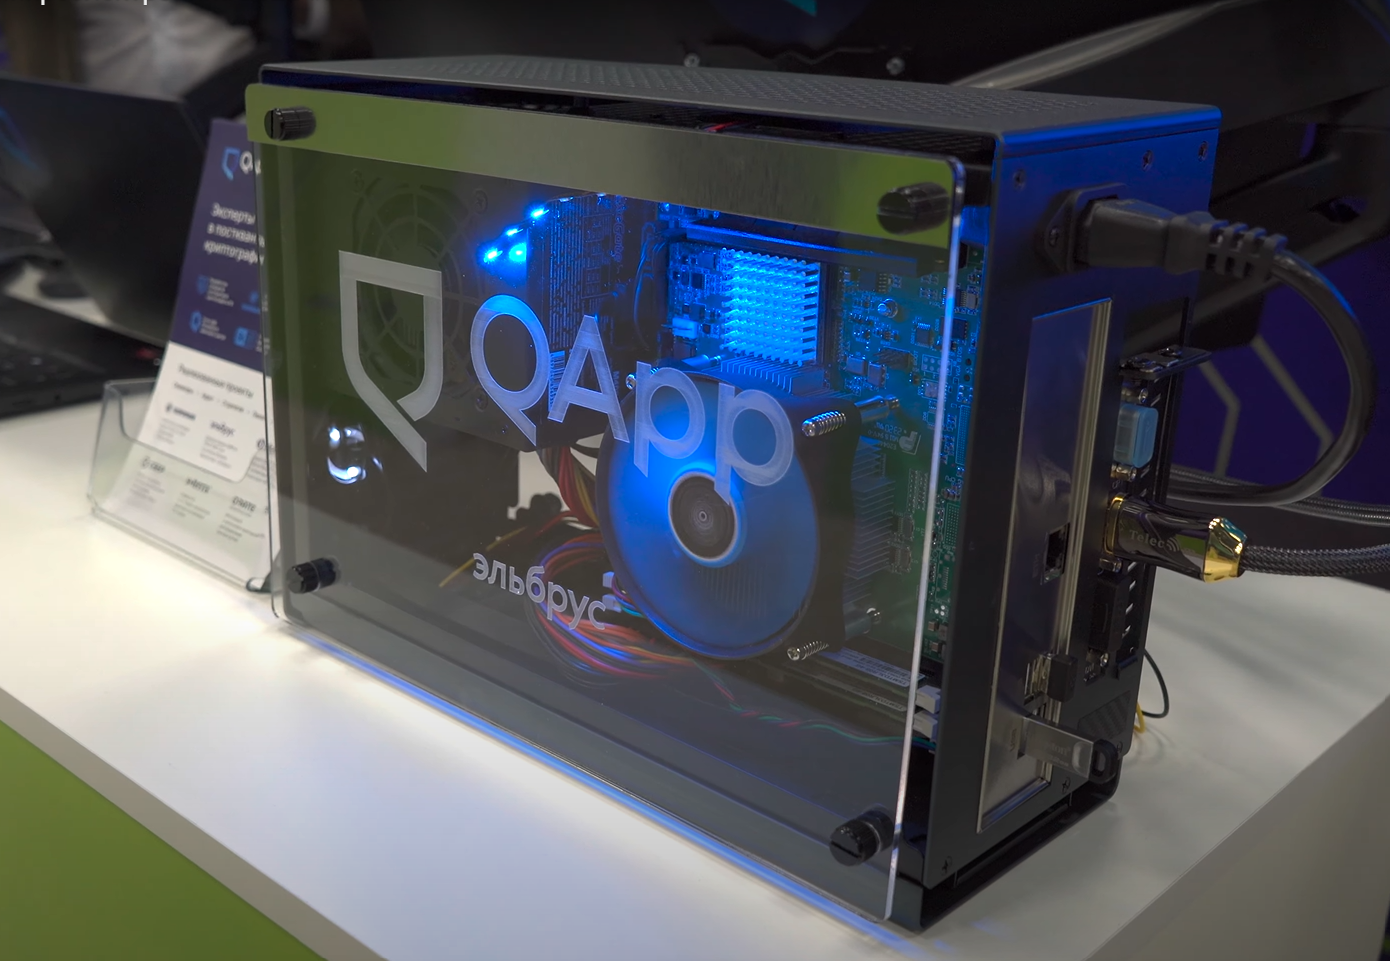
\includegraphics[width=1.0\linewidth]{pics/qapp_x_elbrus.png}
    \caption{Разработка QApp $\times$ Эльбрус. Выставка Микроэлектроника 2022, Сколково}
    \label{qapp}
\end{figure}

Об остальных решениях можно почитать на \href{https://qapp.tech/}{официальном сайте}. 

\subsection{Квантовый центр НИТУ МИСИС}

Научный центр, созданный на базе консорциума НИТУ МИСИС, Российского Квантового Центра, а также ряда инновационных и промышленных предприятий.

Каждый год центр преодолевает несколько технологических барьеров, о чем можно подробно почитать на \href{https://misis.ru/university/struktura-universiteta/centre/90/}{официальном сайте} \href{https://misis.ru/university/struktura-universiteta/centre/90/achievements/}{в разделе "Достижения и перспективы"}.
Отдельно хотелось бы отметить значимые результаты научно-исследовательской деятельности за последние несколько лет:

\begin{figure}[h!]
    \centering
    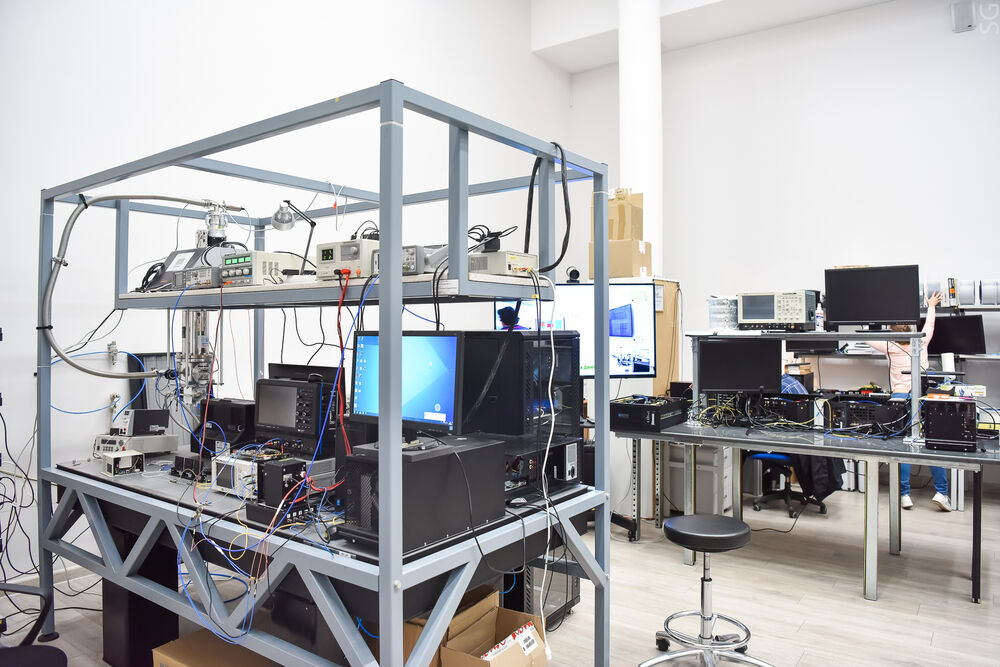
\includegraphics[width=1.0\linewidth]{pics/missis_quantum_centre.jpg}
    \caption{Лаборатория квантового центра НИТУ МИСиС}
    \label{missis_lab}
\end{figure}


\begin{itemize}
    \item Сотрудниками центра разработан экспериментальный образец системы квантового распредления калюча для беспилотных аппаратов. Подобные устройства обеспечат защиту промышленного интернета и беспилотных аппаратов от взлома с применением квантового компьютера.

    \item Создан самый быстрый в России квантовый генератор случайных чисел. Технология может лечь в основу производства коммерческих генераторов случайных чисел, применяемых в криптографии и для моделирования сложных систем.
\end{itemize}

\subsection{ИнфоТеКС}

Лидером в области разработки и производства высокотехнологичных программных и программно-аппаратных средств защиты информации является компания \textbf{ИнфоТеКС}.
Буквально чуть больше месяца назад, 25 октября 2022 года, их квантовая криптографическая система ViPNet QSS выработки и распределения ключей стала первой в России системой, сертифицированной по требованиям ФСБ России.

Немного углубимся в суть данного заголовка и рассмотрим, из чего же состоит данная система. 

\begin{figure}[h!]
    \centering
    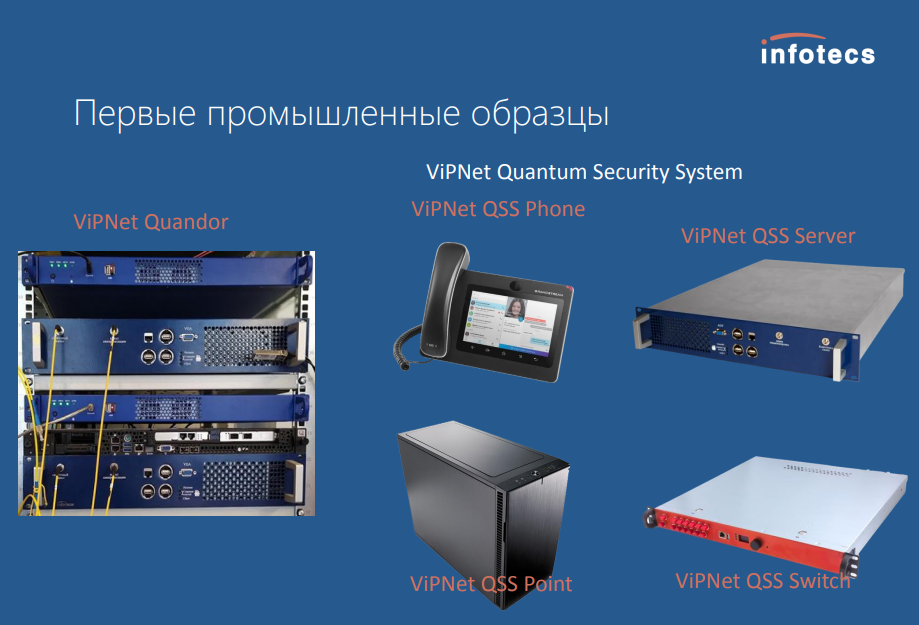
\includegraphics[width=1.0\linewidth]{pics/vipnet_qss.png}
    \caption{Продукты компании infotecs}
    \label{infotecs_product}
\end{figure}

\begin{itemize}
    \item \textbf{ViPNet QSS} - система, предзназначенная для выработки и распределения квантовозащищенных ключей между абонентами, а так же для защиты пользовательского трафика (звонки, аудиосообщения и так далее) между абонентами. 

    \textbf{Особенности:}
    \begin{enumerate}
        \item Данная система позволяет построить сеть кантового распрделения ключей топологии "звезда", к которой может быть поключено $>$ 15000 потребителей квантовозащищенных ключей.
        \item Не подвержена атакам, которые станут возможными при реализации эффективного квантового компьютера.
        \item Стойкость квантового протокола математически доказана.
        \item Шифрование трафика на ключах неизвестных даже администратору сети и так далее\dots
    \end{enumerate}
    
    \item \textbf{Начало разработки}
    
    Разработка началась выработки и распределения ключей началась еще в 2018 году, а уже в мае 2019 был показан действующий образец системы ViPNet QSS Phone, позволявший осуществлять аудиозвонки между абонентами - ``квантовыми'' телефонами ViPNet QSS.
    \item \textbf{Первый реальный проект}
    
    В 2021 году было получено временное разрешение на эксплуатацию системы ViPNet QSS. В декабре 2021 в МГУ им. Ломоносова состоялся запуск \textbf{Университетской Квантовой Сети}. Стоит отметить, что разработка ViPNet QSS - совместный труд компании "ИнфоТеКС" и Центра квантовых технологий физфака МГУ им. Ломоносова. 
    
    Справедливо отметить, что проект УКС обладает большим научным, экспериментальным потенциалом, так как открыт для подключения других вузов, что позволит провести исследования возможностей КРК и квантового оборудования.    
\end{itemize}

\section{Заключение}

Квантовая криптография справедливо считается новым эпохой в эволюции информационной защиты. Именно она позволяет создать практическую абсолютную защиту шифрованных данных от взлома. 

\end{document}